\chapter{Laplace Transform}
Up until this point, the project has focused on the behaviour of electrical circuits in the time domain. Observing how different signals change with time yielded a differential equation, as seen in section (\ref{sec371}).
\\ \\
The solution to a differential equation will often be difficult to derive, and this is where the Laplace transform comes in handy. The Laplace transform converts functions of time to functions of frequency (i.e. from the time domain to the \textit{s}-domain, which is the complex plane that Laplace transforms are graphed on). Since the Laplace transform is an integral transform, the rules of integration can also be applied to the Laplace transform.
\\
\noindent This process reduces the differential equation in question to an algebraic equation. Once the expression has been solved in the \textit{s}-domain, the inverse Laplace transform can be applied to find its corresponding solution in the time domain. Generally, this description can be illustrated in the following way:
\begin{figure}[H]
\center
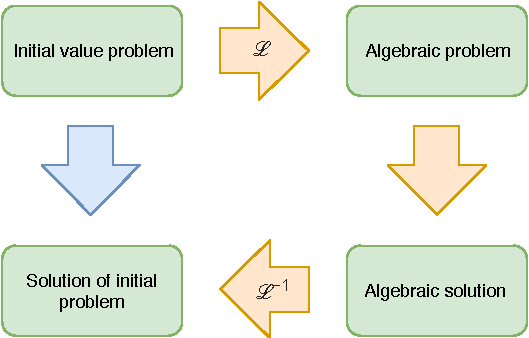
\includegraphics[scale=1]{fig/img/laplace_circ.pdf}
\caption{Visual representation of the concept of the Laplace transform.}
\label{lpsol}
\end{figure}

\section{The Laplace transform}
\begin{definition}{Laplace transform}{lpdef}
For a function of time, $f(t)$, the Laplace transform is $\mathcal{L}\left\{ f(t)\right\} = F(s)$, where $s = \sigma + i\omega$ which is the complex frequency:
\begin{align}
\mathcal{L} \left\{f(t) \right\}=F(s)=\int_{0}^{\infty} e^{-st}\cdot f(t)\ dt.
\end{align}
\end{definition}
\noindent Since the definition consists of an improper integral (where an endpoint approaches some number $c$), it can be rewritten as:
\begin{align}
\int_{0}^{\infty} e^{-st}\cdot f(t)\ dt = \lim_{N \to \infty} \int_{0}^{N} e^{-st}\cdot f(t)\ dt. \label{eq:e(-st)}
\end{align}
When solving equations like \eqref{eq:e(-st)}, it has to be taken into consideration whether the integral converges and diverges. Generally, a function converges when it approaches a specific value. A function diverges when it does not approach a specific value, e.g. when approaching infinity.

\begin{theorem}{Linearity of the Laplace transform}{the:lin_laplace}
The Laplace transform is said to meet the requirements for linearity if:
\begin{align*}
\mathcal{L}\{a\cdot f(t)+b\cdot g(t)\}=a\cdot \mathcal{L}\{f(t)\}+b\cdot \mathcal{L}\{g(t)\},
\end{align*}
where $f$ and $g$ are continuous on a given interval and $a, b \in \mathbb{R}$.
\end{theorem}
\begin{prof}{}{}
The Laplace transform of the function $h(t)=a\cdot f(t)+ b \cdot g(t)$ can be written as follows:
\begin{align*}
\mathcal{L}\{h(t)\}&=\mathcal{L}\{a\cdot f(t)+b\cdot g(t)\},
\\
&=\int_{0}^\infty e^{-st}\left(a\cdot f(t)+b\cdot g(t)\right)dt,
\\
&=\int_{0}^\infty e^{-st}a\cdot f(t)+e^{-st}b\cdot g(t)dt.
\end{align*}
Since integration meets the requirements of linearity, the equation above can be written as the sum of two integral and the constants, $a$ and $b$ can be moved out of the integral:
\begin{align*}
\int_{0}^\infty e^{-st}a\cdot f(t)+e^{-st}b\cdot g(t)dt &=\int_{0}^\infty e^{-st}a\cdot f(t)dt+\int_{0}^\infty e^{-st}b\cdot g(t)dt,
\\
&= a\cdot \int_{0}^\infty e^{-st} f(t)dt+\cdot b \int_{0}^\infty e^{-st} g(t)dt.
\end{align*}
From \Cref{the:lin_laplace}, this can written as the sum of two Laplace transforms:
\begin{align*}
a\cdot \int_{0}^\infty e^{-st} f(t)dt+\cdot b \int_{0}^\infty e^{-st} g(t)dt =a\cdot \mathcal{L}\{f(t)\}+b\cdot \mathcal{L}\{g(t)\}.
\end{align*}
\end{prof}
\begin{theorem}{Existence of the Laplace transform}{geqleq}

The function $f$ is said to be of exponential order if there exist nonnegative constants $M$, $c$, and $T$  such that $$|f(t)| \leq Me^{ct},    \text{   for } t \geq T.$$
Thus a function is of exponential order provided that it grows no more rapidly than a constant multiple of some exponential function with a linear exponent. \cite[p. 320]{diffandcomplex}
\end{theorem}
\begin{prof}{}{}
Since $f$ is of exponential order, then $|f(t)| \leq Me^{ct}$ for all $t \geq 0$. Note that since $s$ is a complex number  $s=\sigma+i\omega$, it can be divided into its real and imaginary parts. It then follows that: $$\lim_{N \to \infty} \int_{0}^{N} |f(t)e^{-st}|\ dt = \lim_{N \to \infty} \int_{0}^{N} |f(t)| |e^{-i\omega t}|e^{-\sigma t}\ dt.$$
By \Cref{complex:exp:eq}, the complex number $s$ can also take the form: 
$$e^{\sigma}e^{i\omega}= e^{\sigma}(\cos(\omega)+i\sin(\omega)).$$
Since the imaginary parts are defined as functions of cosine and sine, they can not approach $\infty$. Then naturally $|e^{i\omega t}|=1$ for all $\omega \in \mathbb{R}$. This now yields: $$\lim_{N \to \infty} \int_{0}^{N} |f(t)e^{-\sigma t}|\ dt \leq \lim_{N \to \infty} \int_{0}^{N} Me^{ct}e^{-\sigma t}\ dt = M \lim_{N \to \infty} \int_{0}^{N}e^{-(c-\sigma)t}\ dt. $$ The integral is only going to converge when $(c-\sigma)>0$ or Re$(s)>c$.
\end{prof}

\begin{example}{Laplace transform for $k$}{lpone}
From \Cref{lpdef}, let $f(t)=k$ where $k$ is a constant. In that case:
\begin{align*}
\mathcal{L}\{k\}=\int_{0}^{\infty} e^{-st} \cdot k\ dt.
\end{align*}
Now $\infty$ is replaced with some value $N$ that is set to approach $\infty$:
\begin{align*}
\mathcal{L} \left\{k \right\}= \lim_{N \to \infty} k\cdot \int_{0}^{N} e^{-st}\ dt.
\end{align*}
$e^{-st}$ is now integrated with respect to $t$:
\begin{align*}
\mathcal{L} \left\{k \right\}= \lim_{N \to \infty} \left[ -\dfrac{k}{s} e^{-st} \right]_{0}^{N}.  
\end{align*}
Zero and $N$ are now inserted in place of $t$:
\begin{align*}
\mathcal{L} \left\{k \right\}= \lim_{N \to \infty} \left( -\dfrac{k}{s} e^{-sN} - \left(-\dfrac{k}{s}\right) \right).
\end{align*}
Now observe what happens when $N$ approaches $\infty$:
\begin{align*}
\mathcal{L} \left\{k \right\}=\dfrac{k}{s} \ \ \ ; \ \ \ Re(s) > 0.
\end{align*}
Here the real part of $s$ has to be greater than zero, hence it makes $-\dfrac{k}{se^{sN}}$ converge towards zero. If it is less than zero the expression would start to diverge, and would therefore not make sense to look at.
\end{example}

\begin{example}{Laplace transform for $e^{at}$}{lpe}
From \Cref{lpdef}, let $f(t)=e^{at}$, where $a$ is a constant, and $t$ is time. In that case:
$$\mathcal{L} \left\{e^{at} \right\}=\int_{0}^{\infty} e^{-st}\cdot e^{at}\ dt.$$
Since they have the base, $e$, in common, their exponents can be combined. Additionally, $t$ can be factorised:
$$\mathcal{L} \left\{e^{at} \right\}=\int_{0}^{\infty} e^{-(s-a)t}\ dt.$$
Integration by substitution is now applied. Let $u = -(s-a)t$, then $\dfrac{du}{dt}=-(s-a)$. This yields $dt=-\dfrac{1}{s-a}du$. The integral is now no longer from 0 to $\infty$, since new limits are applied. It is now an integral from $u \cdot 0=-(s-a)0=0$ to $u\cdot N=-(s-a)N$. Since $-\dfrac{1}{s-a}$ is a constant it can be moved outside the integral. Thus:
\begin{align}
\mathcal{L}\{e^{at}\}=\lim_{N \to \infty} \int_{0}^{-(s-a)N} e^{u}\cdot -\dfrac{1}{s-a}\ du = \lim_{N \to \infty} -\dfrac{1}{s-a} \cdot \left[e^{u} \right]_{0}^{-(s-a)N}.
\label{eq6.2}
\end{align}
Then evaluating the integral at the boundaries:
\begin{align*}
\mathcal{L} \left\{e^{at} \right\} =\lim_{N \to \infty} -\dfrac{1}{s-a}\cdot (e^{-(s-a)N}-e^{0}).
\end{align*}
When $N$ is approaching $\infty$ (if $Re(s) \geq a$), $e^{-(s-a)N}$ will approach $0$. Therefore the equation is going to look as follows:
\begin{align*}
\mathcal{L} \left\{e^{at} \right\} = \dfrac{1}{s-a}.
\end{align*}
In conclusion, the Laplace transform of $f(t)=e^{at}$ equals:
$$\mathcal{L} \left\{e^{at} \right\} =\dfrac{1}{s-a} \ \ \ ;\ \ \ Re(s)>a.$$
$s$ must be greater than $a$, since the limit of $e^{-(s-a)N}$ converges towards zero. If $a$ is greater than $s$, the exponent of $e$ would be positive, and the limit would diverge.
\end{example}
%The Laplace transform can be used for all functions of $f$, where the real part of $s$ is greater than $a$ $Re(s) \geq a$. Since $s$ is a complex number ($s=a+ib$), only the first part of $s$ has to be greater than $a$. Therefore, $e^{-st}$ is  the same as $e^{-ta}e^{-tib}$, where the last part is the imaginary part of the complex number. In the complex chapter, this is also defined as $e^{a}\cos(b)+ i \sin(b)$.% 
\noindent When doing the inverse Laplace transform, the results can often be found by looking at the results from on ordinary Laplace transform, because $F(s) = \mathcal{L}\left\{f(t)\right\} \Rightarrow\mathcal{L}^{-1}\big\{ F(s)\big\} = f(t)$.
\begin{example}{Inverse Laplace transform}{}
Let $F(s) = \dfrac{4}{s+10}$. When recognizing this takes the same form as the result above, the solution becomes clear. Now this has to be put on the form $f(t)=e^{at}$, where, in this case, the constant is 10. The result is therefore:
\begin{align*}
\mathcal{L}^{-1} \left\{F(s) \right\} = 4e^{-10t}.
\end{align*}
\end{example}
\noindent The Laplace transform can be applied to the derivatives of multiple orders. In particular, the Laplace transform of the first order derivative, since it is essential when looking at the high- and low-pass filters.
%mere tekst/bedre overgang
\begin{theorem}{Laplace transform of a first order derivative}{theorem:lap_diff}
The Laplace-transform of a first order derivative takes the following form:
$$\mathcal{L} \left\{\frac{df}{dt} \right\} = s \cdot F(s)-f(0).$$
\end{theorem}
\noindent The Laplace transform of the first derivative is using the rule of integration by parts. The rule states the following:
\begin{align}
\int_{a}^{b}{u(t) \cdot \dfrac{dv}{dt}dt}=\left[u(t) \cdot v(t) \right]_{a}^{b}-\int_{a}^{b} \frac{du}{dt}\cdot v(t) dt.
\label{eq:intbyparts}
\end{align}
\begin{prof}{Laplace transform of a first order derivative}{lpderiv}
From \Cref{lpdef}, $u(t)$ and $v(t)$ from \eqref{eq:intbyparts} are given by: $u(t) = e^{-st}$ and $v(t) = f(t)$. Furthermore, infinity is replaced with the limit of some value N approaching $\infty$. This yields:
$$\mathcal{L} \left\{\frac{df}{dt} \right\}=\lim_{N \to \infty} \left(\left[e^{-st}\cdot f(t)\right]_{0}^{N}-\int_{0}^{N} -s\cdot e^{-st}\cdot f(t)\ dt \right).$$
Because $s$ is merely a constant, it can be placed outside of the integral, such that:
\begin{align}
\mathcal{L} \left\{\frac{df}{dt} \right\}=\lim_{N \to \infty} \left[\dfrac{1}{e^{st}}\cdot f(t)\right]_{0}^{N}+ s \cdot \lim_{N \to \infty} \left( \int_{0}^{N}e^{-st}\cdot f(t)\ dt \right).\label{eq:Lderivative1}
\end{align}
Note that the second term of \eqref{eq:Lderivative1} now equals the product of $s$ and $\mathcal{L}\{f(t)\}$:
\begin{align}
\mathcal{L} \left\{\frac{df}{dt} \right\} = \lim_{N \to \infty}\left[\dfrac{1}{e^{s\cdot N}}\cdot f(N)-\dfrac{1}{e^{s\cdot 0}}\cdot f(0)\right]+s\cdot \mathcal{L} \left\{f(t) \right\}. \label{eq:lap:dfdt}
\end{align}
From \Cref{geqleq}, it follows that the first term in \eqref{eq:lap:dfdt} approaches $0$ if:
\begin{align*}
\lim_{N \to \infty} e^{-s\cdot N}\cdot f(N) &\leq \lim_{N \to \infty} e^{-s\cdot N} Me^{c\cdot N},\\
&\leq M \cdot \lim_{N \to \infty} e^{(c-s)N},
\end{align*}
if $Re(s) > c$.
$$\mathcal{L} \left\{\frac{df}{dt} \right\} = \left[0-\dfrac{f(0)}{1}\right]+s\cdot \mathcal{L} \left\{f(t) \right\}.$$
This can be rearranged to the following:
\begin{align*}
\mathcal{L} \left\{\frac{df}{dt} \right\} = s\cdot \mathcal{L}\{f(t)\}-f(0).
\end{align*}

\end{prof}
\begin{table}[H]
\center
\begin{tabular}{lll}
\hline
\multicolumn{1}{|l|}{$f(t)$}           & \multicolumn{1}{l|}{$F(s)$}                & \multicolumn{1}{l|}{Limits}    \\ \hline
\multicolumn{1}{|l|}{$k$}              & \multicolumn{1}{l|}{$\dfrac{k}{s}$}        & \multicolumn{1}{l|}{$Re(s)>0$} \\ \hline
\multicolumn{1}{|l|}{$e^{at}$}         & \multicolumn{1}{l|}{$\dfrac{1}{s-a}$}      & \multicolumn{1}{l|}{$Re(s)>a$} \\ \hline
\multicolumn{1}{|l|}{$\dfrac{df}{dt}$} & \multicolumn{1}{l|}{$s \cdot F(s) - f(0)$} & \multicolumn{1}{l|}{$Re(s)>0$} \\ \hline                          
\end{tabular}
\caption{Table of Laplace transforms.}
\label{lptable}
\end{table}
\noindent To fully understand the concept behind figure \ref{lpsol}, an example of finding the solution of a differential equation will be solved using the Laplace transform. Differential equations can be difficult to solve without the Laplace transform, but can be solved using the Laplace transform. A table with the results from the previous examples and proofs is constructed above.

\begin{example}{Laplace example}{laplaceexample}
In this example the following differential equation will be solved using the Laplace transform:
\begin{align}
\dfrac{df}{dt}-4f(t)=e^{6t}, \label{eq:lap_ex}
\end{align} 
with the initial condition $f(0)=-2$. The Laplace transform is applied on both sides (constants can be moved outside as stated in \cref{the:lin_laplace}:
\begin{align*}
\mathcal{L} \left\{\dfrac{df}{dt} \right\}-4 
\mathcal{L} \left\{f(t) \right\} = 
\mathcal{L} \left\{e^{6t} \right\}.
\end{align*}
The Laplace transforms from table \ref{lptable} imply:
\begin{align*}
s \cdot F(s) - f(0) - 4F(s)= \dfrac{1}{s-6}.
\end{align*}
Now $f(0)=-2$ is inserted:
\begin{align*}
s \cdot F(s) + 2 - 4F(s)= \dfrac{1}{s-6}.
\end{align*}
$-2$ is now subtracted from both sides and put on a common denominator:
\begin{align*}
s \cdot F(s) - 4F(s)= \dfrac{1-2(s-6)}{s-6}.
\end{align*}
$F(s)$ is factorised on the left side:
\begin{align*}
F(s) \cdot (s-4) = \dfrac{1-2(s-6)}{s-6}.
\end{align*}
Both sides are now divided by $s-4$ and the numerator on the right side is simplified:
\begin{align*}
F(s) = \dfrac{13-2s}{(s-6)(s-4)}.
\end{align*}
Now the next step is to find the inverse Laplace transform. This is done using partial-fraction decomposition: \cite[p. 537]{calc}
\begin{align}
F(s) = \dfrac{13-2s}{(s-6)(s-4)} = A \dfrac{1}{s-6} + B \dfrac{1}{s-4}.
\label{par_dec}
\end{align}
Both sides of the expression above are now multiplied with the denominator of the left-hand side $((s-6)(s-4))$:
\begin{align*}
13-2s = A(s-4) + B(s-6).
\end{align*}
Now this is split up in elements that are multiplied by $s$ and elements which are not:
\begin{align*}
13-2s = s(A+B)+(-4A-6B).
\end{align*}
Now two equations with two unknown variables are created:
\begin{align*}
A+B &=-2 \Leftrightarrow A=-2-B, \\
-4A-6B &=13 \Leftrightarrow -4(-2-B)-6B = 13 \Leftrightarrow 8 + 4B - 6B = 13 \Leftrightarrow -2B = 5 \Leftrightarrow B = -\dfrac{5}{2}.
\end{align*}
The $B$ value is inserted to find $A$:
\begin{align*}
A=-2- \left(-\dfrac{5}{2} \right), \\
A=\dfrac{1}{2}.
\end{align*}
These values are now inserted into \eqref{par_dec}:
\begin{align*}
F(s) = \dfrac{1}{2} \cdot \dfrac{1}{s-6} - \dfrac{5}{2} \cdot \dfrac{1}{s-4}.
\end{align*}
The inverse Laplace transform is now applied. Since it is possible to treat the Laplace transform as an integral, constants are moved outside the transform, as stated in \Cref{the:lin_laplace}:
\begin{align*}
\mathcal{L}^{-1} \left\{F(s) \right\} = \dfrac{1}{2} \cdot \mathcal{L}^{-1} \left\{\dfrac{1}{s-6} \right\} - \dfrac{5}{2} \cdot \mathcal{L}^{-1} \left\{\dfrac{1}{s-4} \right\}.
\end{align*}
Now the solutions can be identified from table \ref{lptable}:
\begin{align*}
f(t) = \dfrac{1}{2} \cdot e^{6t} - \dfrac{5}{2}e^{4t}.
\end{align*}
This result can be tested by inserting the values into \eqref{eq:lap_ex}:
\begin{align*}
\dfrac{df}{dt} \left(\dfrac{1}{2} \cdot e^{6t} - \dfrac{5}{2}e^{4t} \right) - 4 \cdot \left(\dfrac{1}{2} \cdot e^{6t} - \dfrac{5}{2}e^{4t} \right) &= e^{6t}, \\
\left(\dfrac{1}{2} \cdot \left(\dfrac{df}{dt} \left(e^{6t} \right) \right) - \dfrac{5}{2} \cdot \left(\dfrac{df}{dt} \left(e^{4t} \right) \right) \right) - 4 \cdot \left(\dfrac{1}{2} \cdot e^{6t} - \dfrac{5}{2} e^{4t} \right) &= e^{6t}, \\
\left(\dfrac{1}{2} \left(6e^{6t} \right) - \dfrac{5}{2} \left(4e^{4t} \right) \right) - \dfrac{4}{2}e^{6t}+\dfrac{20}{2}e^{4t}&= e^{6t},\\
3e^{6t}-10e^{4t}-2e^{6t}+10e^{4t} &= e^{6t}, \\
e^{6t} &= e^{6t}.
\end{align*}
Hereby the solution to the \eqref{eq:lap_ex} is found using the Laplace transform.
\end{example}